\documentclass[tikz,border=5mm]{standalone}
\begin{document}
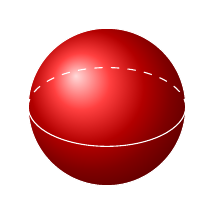
\begin{tikzpicture}
    % 绘制球体
    \shade[ball color=red] (0,0) circle (1cm);
    
    % 绘制高光
%    \fill[white] (0.2,0.2) circle (0.2cm);
    
    % 绘制赤道和子午线
    \draw [white] (0,0) circle (1cm);
    \draw [white] (-1,0) arc (180:360:1cm and 0.5cm);
    \draw[dashed, white] (1,0) arc (0:180:1cm and 0.5cm);
    
    % 标注球心
%    \node [circle,fill=black,inner sep=1pt,label=below:$O$] at (0,0) {};
\end{tikzpicture}
\end{document}